\subsection{Additional Graph Definitions}
\label{sec:future-graphs}

This section defines two graph constructions that require data sources beyond a single commit snapshot: the co-modification graph (\S\ref{sec:co-edit-graph}), which captures logical coupling from version control history, and the temporal graph sequence (\S\ref{sec:temporal-graphs}), which enables longitudinal structural analysis.

\subsubsection{The File Co-Modification Graph}
\label{sec:co-edit-graph}

The module graph captures \emph{structural coupling} (explicit import dependencies), but software engineering research has long recognized a complementary form of coupling: \emph{logical coupling}, measured by co-modification frequency in version control~\cite{decan2019}. Two modules that are frequently modified together---even without a direct import relationship---likely share a hidden dependency that the import graph does not capture.

\begin{definition}[Co-modification graph]\label{def:co-edit-graph}
Let $\{p_1, \ldots, p_R\}$ be the set of merged pull requests to \module{Mathlib} over a given time window. For each PR~$p_r$, let $\mathrm{files}(p_r) \subseteq \mathcal{M}$ be the set of modules modified. The \emph{co-modification graph} is the weighted undirected graph
\[
  G_{\mathrm{co}} = (\mathcal{M},\, E_{\mathrm{co}},\, w_{\mathrm{co}}), \quad w_{\mathrm{co}}(m_i, m_j) = |\{p_r : m_i, m_j \in \mathrm{files}(p_r)\}|.
\]
An edge exists between $m_i$ and $m_j$ if $w_{\mathrm{co}}(m_i, m_j) \ge 1$.
\end{definition}

\begin{figure}[!htb]
\centering
\begin{subfigure}[t]{0.46\textwidth}
\centering
\vspace{0pt}
\raggedright\scriptsize\ttfamily
\textsf{\bfseries\color{gray!70}PR \#18042}\textsf{\color{gray!50}\enspace``refactor Nat order lemmas''}\\[2pt]
\hspace{1em}\textcolor{blue!60!black}{Data/Nat/Defs.lean}\\
\hspace{1em}\textcolor{blue!60!black}{Data/Nat/Order.lean}\\
\hspace{1em}\textcolor{blue!60!black}{Data/Int/Defs.lean}\\[8pt]
\textsf{\bfseries\color{gray!70}PR \#18107}\textsf{\color{gray!50}\enspace``add Int.cast lemmas''}\\[2pt]
\hspace{1em}\textcolor{blue!60!black}{Data/Nat/Defs.lean}\\
\hspace{1em}\textcolor{blue!60!black}{Data/Int/Defs.lean}\\[8pt]
\textsf{\bfseries\color{gray!70}PR \#18253}\textsf{\color{gray!50}\enspace``move group lemmas''}\\[2pt]
\hspace{1em}\textcolor{blue!60!black}{Algebra/Group/Defs.lean}\\
\hspace{1em}\textcolor{blue!60!black}{Data/Nat/Order.lean}\\[8pt]
\textnormal{\sffamily Co-modification counts:}\\[2pt]
\hspace{1em}\textnormal{\sffamily\tiny%
Nat.Defs $\leftrightarrow$ Int.Defs: 2 PRs,\quad
Nat.Defs $\leftrightarrow$ Nat.Order: 1,}\\
\hspace{1em}\textnormal{\sffamily\tiny%
Int.Defs $\leftrightarrow$ Nat.Order: 1,\quad
Group.Defs $\leftrightarrow$ Nat.Order: 1}
\caption{Three PRs and the modules they touch. Pairs co-modified in multiple PRs get higher weight.}
\label{fig:co-edit-source}
\end{subfigure}%
\hfill
\begin{subfigure}[t]{0.50\textwidth}
\centering
\vspace{0pt}
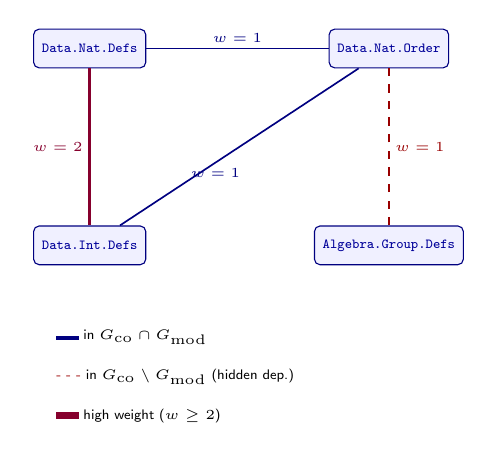
\begin{tikzpicture}[
  every node/.style={font=\scriptsize, inner sep=2pt},
  mod/.style={rounded corners=2pt, draw=blue!50!black, fill=blue!6,
    font=\tiny\ttfamily, text=blue!60!black, inner sep=3pt, minimum height=14pt},
  coedge/.style={-, blue!50!black, semithick},
  strongedge/.style={-, purple!70!black, very thick},
  hiddenedge/.style={-, red!60!black, semithick, dashed},
]
  % Nodes
  \node[mod] (natd) at (0, 2.5) {Data.Nat.Defs};
  \node[mod] (nato) at (3.8, 2.5) {Data.Nat.Order};
  \node[mod] (intd) at (0, 0) {Data.Int.Defs};
  \node[mod] (grpd) at (3.8, 0) {Algebra.Group.Defs};
  % Edges with weights
  % Strong edge: co-modified 2 times
  \draw[strongedge] (natd) -- node[left, font=\tiny\sffamily, text=purple!70!black] {$w=2$} (intd);
  % Normal edges: co-modified 1 time, also in G_module
  \draw[coedge] (natd) -- node[above, font=\tiny\sffamily, text=blue!50!black] {$w=1$} (nato);
  \draw[coedge] (intd) -- node[below, font=\tiny\sffamily, text=blue!50!black, pos=0.4] {$w=1$} (nato);
  % Hidden dependency: co-modified but NOT in G_module
  \draw[hiddenedge] (grpd) -- node[right, font=\tiny\sffamily, text=red!60!black] {$w=1$} (nato);
  % Legend
  \node[font=\tiny\sffamily, anchor=north west] at (-0.5, -1.0)
    {\textcolor{blue!50!black}{\rule{8pt}{1.5pt}} in $G_{\mathrm{co}} \cap G_{\mathrm{mod}}$};
  \node[font=\tiny\sffamily, anchor=north west] at (-0.5, -1.5)
    {\textcolor{red!60!black}{- - -} in $G_{\mathrm{co}} \setminus G_{\mathrm{mod}}$ (hidden dep.)};
  \node[font=\tiny\sffamily, anchor=north west] at (-0.5, -2.0)
    {\textcolor{purple!70!black}{\rule{8pt}{2.5pt}} high weight ($w \ge 2$)};
\end{tikzpicture}
\caption{$G_{\mathrm{co}}$: edge weight = number of PRs co-modifying both modules. The \textcolor{red!60!black}{dashed edge} has no import in $G_{\mathrm{mod}}$---a hidden dependency.}
\label{fig:co-edit-graph}
\end{subfigure}
\caption{Co-modification graph (Definition~\ref{def:co-edit-graph}). (a)~Three merged PRs and the files each touches. (b)~The resulting weighted undirected graph $G_{\mathrm{co}}$: \textcolor{blue!50!black}{solid} edges exist in both $G_{\mathrm{co}}$ and $G_{\mathrm{mod}}$ (structural + logical coupling); the \textcolor{red!60!black}{dashed} edge between \module{Algebra.Group.Defs} and \module{Data.Nat.Order} appears only in $G_{\mathrm{co}}$, revealing a hidden dependency invisible to the import graph. The \textcolor{purple!70!black}{thick} edge ($w=2$) indicates a stronger coupling. All names have the \module{Mathlib.}\ prefix removed.}
\label{fig:co-modification}
\end{figure}

This graph captures traces of \emph{human organizational process} from a data source entirely independent of Lean's compilation model: the Git history. Comparing $G_{\mathrm{co}}$ with $G_{\mathrm{module}}$ tests whether structural coupling predicts logical coupling. Module pairs with high co-modification weight but no direct import edge reveal hidden dependencies---candidates for refactoring or explicit import addition. Conversely, direct import edges with zero co-modification suggest stable, well-encapsulated interfaces.

\subsubsection{Temporal Graph Sequences}
\label{sec:temporal-graphs}

All analyses in this paper are computed from a single snapshot. A longitudinal extension would test whether the structural properties we observe are stable invariants of mathematical content or transient features of a particular development phase.

\begin{definition}[Temporal graph sequence]\label{def:temporal-sequence}
Let $\{c_1, c_2, \ldots, c_T\}$ be a sequence of $T$ historical \module{Mathlib} commits. Each commit $c_t$ yields an environment $\mathcal{E}_t$ and corresponding graphs $G_{\mathrm{thm}}^{(t)} = (\mathcal{D}_t, E_t)$ and $G_{\mathrm{mod}}^{(t)} = (\mathcal{M}_t, F_t)$. Define:
\begin{itemize}
  \item \emph{Growth indicators}: $|\mathcal{D}_t|$, $|\mathcal{M}_t|$, and edge density $|E_t| / |\mathcal{D}_t|$.
  \item \emph{Structural stability}: community persistence $\mathrm{NMI}(\mathcal{L}^{(t)}, \mathcal{L}^{(t+1)})$, hub turnover (rank correlation of in-degree rankings between consecutive snapshots), and redundancy trend $r(G_{\mathrm{mod}}^{(t)})$ over time.
  \item \emph{Structural events}: discontinuities in the time series coinciding with known events (e.g., the Lean~3$\to$4 port via Mathport, 2023; the module system introduction, November 2025).
\end{itemize}
\end{definition}

\begin{figure}[!htb]
\centering
\begin{subfigure}[t]{0.38\textwidth}
\centering
\vspace{0pt}
\raggedright\scriptsize
\textsf{\bfseries Timeline of snapshots}\\[6pt]
\begin{tikzpicture}[
  every node/.style={font=\tiny\sffamily},
  dot/.style={circle, fill=blue!60!black, minimum size=3pt, inner sep=0pt},
  event/.style={font=\tiny\sffamily\itshape, text=red!60!black},
]
  % Timeline
  \draw[->, >=Stealth, gray!60, thick] (0, 0) -- (0, -5.2);
  \node[font=\tiny\sffamily, gray!50, anchor=east] at (-0.15, 0) {$t$};
  % Snapshots
  \node[dot] (c1) at (0, -0.3) {};
  \node[anchor=west] at (0.2, -0.3) {$c_1$: Jan 2023};
  \node[dot] (c2) at (0, -1.2) {};
  \node[anchor=west] at (0.2, -1.2) {$c_2$: Jul 2023};
  \node[event, anchor=west] at (0.2, -1.55) {Lean 3$\to$4 port};
  \node[dot] (c3) at (0, -2.4) {};
  \node[anchor=west] at (0.2, -2.4) {$c_3$: Jan 2024};
  \node[dot] (c4) at (0, -3.3) {};
  \node[anchor=west] at (0.2, -3.3) {$c_4$: Jan 2025};
  \node[dot] (c5) at (0, -4.2) {};
  \node[anchor=west] at (0.2, -4.2) {$c_5$: Nov 2025};
  \node[event, anchor=west] at (0.2, -4.55) {module system};
  \node[dot, fill=orange!80!red] (c6) at (0, -5.0) {};
  \node[anchor=west, text=orange!80!red] at (0.2, -5.0) {$c_T$: Feb 2026 (this paper)};
\end{tikzpicture}
\caption{Monthly snapshots $\{c_1, \ldots, c_T\}$ with structural events marked.}
\label{fig:temporal-timeline}
\end{subfigure}%
\hfill
\begin{subfigure}[t]{0.58\textwidth}
\centering
\vspace{0pt}
\begin{tikzpicture}[
  every node/.style={font=\scriptsize, inner sep=2pt},
  mod/.style={circle, fill=blue!60!black, minimum size=2.5pt, inner sep=0pt},
  edge/.style={-, blue!30!black, semithick, opacity=0.5},
  frame/.style={rounded corners=3pt, draw=gray!40, fill=gray!3, inner sep=4pt},
]
  % Graph at t=1 (small)
  \node[frame, minimum width=50pt, minimum height=40pt] (f1) at (0, -0.5) {};
  \node[font=\tiny\sffamily, gray!60, above=0pt of f1] {$G^{(c_1)}$};
  \node[mod] (a1) at (-0.4, -0.2) {};
  \node[mod] (b1) at (0.3, -0.1) {};
  \node[mod] (c1n) at (-0.1, -0.7) {};
  \node[mod] (d1) at (0.5, -0.8) {};
  \draw[edge] (a1) -- (b1);
  \draw[edge] (b1) -- (c1n);
  \draw[edge] (c1n) -- (d1);
  % Growth indicators
  \node[font=\tiny\sffamily, text=gray!50, below=2pt of f1] {$|\mathcal{D}|{=}50\text{k}$};
  % Graph at t=3 (medium)
  \node[frame, minimum width=55pt, minimum height=45pt] (f3) at (2.3, -0.5) {};
  \node[font=\tiny\sffamily, gray!60, above=0pt of f3] {$G^{(c_3)}$};
  \node[mod] (a3) at (1.8, -0.1) {};
  \node[mod] (b3) at (2.5, 0.0) {};
  \node[mod] (c3n) at (2.0, -0.5) {};
  \node[mod] (d3) at (2.7, -0.4) {};
  \node[mod] (e3) at (2.3, -0.9) {};
  \node[mod] (f3n) at (1.9, -0.9) {};
  \draw[edge] (a3) -- (b3);
  \draw[edge] (a3) -- (c3n);
  \draw[edge] (b3) -- (d3);
  \draw[edge] (c3n) -- (e3);
  \draw[edge] (d3) -- (e3);
  \draw[edge] (c3n) -- (f3n);
  \node[font=\tiny\sffamily, text=gray!50, below=2pt of f3] {$|\mathcal{D}|{=}150\text{k}$};
  % Graph at t=T (large, current)
  \node[frame, minimum width=62pt, minimum height=50pt, draw=orange!60!red] (fT) at (4.8, -0.5) {};
  \node[font=\tiny\sffamily, orange!80!red, above=0pt of fT] {$G^{(c_T)}$};
  \node[mod, fill=orange!80!red] (aT) at (4.3, 0.0) {};
  \node[mod, fill=orange!80!red] (bT) at (5.0, 0.1) {};
  \node[mod, fill=orange!80!red] (cT) at (4.5, -0.3) {};
  \node[mod, fill=orange!80!red] (dT) at (5.2, -0.3) {};
  \node[mod, fill=orange!80!red] (eT) at (4.3, -0.7) {};
  \node[mod, fill=orange!80!red] (fT2) at (4.8, -1.0) {};
  \node[mod, fill=orange!80!red] (gT) at (5.3, -0.7) {};
  \node[mod, fill=orange!80!red] (hT) at (4.6, -0.5) {};
  \draw[-, orange!40!red, semithick, opacity=0.5] (aT) -- (bT);
  \draw[-, orange!40!red, semithick, opacity=0.5] (aT) -- (cT);
  \draw[-, orange!40!red, semithick, opacity=0.5] (bT) -- (dT);
  \draw[-, orange!40!red, semithick, opacity=0.5] (cT) -- (eT);
  \draw[-, orange!40!red, semithick, opacity=0.5] (dT) -- (gT);
  \draw[-, orange!40!red, semithick, opacity=0.5] (eT) -- (fT2);
  \draw[-, orange!40!red, semithick, opacity=0.5] (hT) -- (fT2);
  \draw[-, orange!40!red, semithick, opacity=0.5] (cT) -- (hT);
  \draw[-, orange!40!red, semithick, opacity=0.5] (gT) -- (fT2);
  \node[font=\tiny\sffamily, text=orange!80!red, below=2pt of fT] {$|\mathcal{D}|{=}318\text{k}$};
  % Growth arrows
  \draw[->, >=Stealth, gray!40, thick] (0.95, -0.5) -- (1.55, -0.5);
  \node[font=\tiny\sffamily, gray!40, above] at (1.25, -0.5) {$\cdots$};
  \draw[->, >=Stealth, gray!40, thick] (3.15, -0.5) -- (3.95, -0.5);
  \node[font=\tiny\sffamily, gray!40, above] at (3.55, -0.5) {$\cdots$};
  % Tracked metrics below
  \node[font=\tiny\sffamily, anchor=north west] at (-0.8, -2.0)
    {Track: $|\mathcal{D}_t|$, edge density, community NMI, hub turnover, redundancy $r(G_{\mathrm{mod}}^{(t)})$};
\end{tikzpicture}
\caption{Graph snapshots growing over time; structural metrics tracked across the sequence detect events and trends.}
\label{fig:temporal-graph}
\end{subfigure}
\caption{Temporal graph sequence (Definition~\ref{def:temporal-sequence}). (a)~Monthly snapshots of \module{Mathlib} commits, with two structural events: the Lean~3$\to$4 port (2023) and the module system introduction (November 2025). (b)~The declaration graph $G_{\mathrm{thm}}^{(t)}$ at three time points, growing from ${\sim}50$k to $318$k declarations. Tracking structural indicators across the sequence reveals whether properties like the $17.5\%$ redundancy rate are stable invariants or transient features of a particular development phase.}
\label{fig:temporal-sequence}
\end{figure}

The temporal dimension directly captures the \emph{process} of organizational restructuring. If \module{Mathlib}'s dependency structure is primarily determined by inherited mathematical logic, structural indicators should be stable under refactoring; if organizational process dominates, we expect significant structural change at refactoring events while mathematical content remains constant. The Lean~3$\to$4 port is a natural experiment: identical mathematical content, entirely rewritten proof infrastructure.
